% !TEX root = ../master.tex
\chapter{Implementation and Evaluation}
\label{chap:impl}

In this chapter the implementation of the two artifacts identified and designed in the previous chapter is executed.
First, an attempt is made to implement the visual volume detection system and test it out in a real-world test environment.
Then simulation of an elevator system is implemented to compare tree scheduling strategies and the results of this simulation are evaluated.


\section{Visual System}
TODO
\subsection{Implementation with OpenCV and Python}

The implementation is written in Python 3 in version 3.6 \autocite[][]{python2018python366}
with bindings to OpenCV 3.4.2.
Python was chosen as the implementation language, since it provides a higher abstraction and better ergonomics than C++.
Furthermore, the author is proficient in it.

There exists a C++ implementation of a perspective correct volume intersection, which however is used for a more detailed reconstruction of a small statue, which is photographed 36 times and rotated around its own axis \autocite[][]{xocoatzin2013voxelcarving}.
This C++ implementation gave a first reference for the implementation in Python.

follows approach up to volume reconstruction, which however is done orthographically
main program in \ref{lst:app:volmain} in appendix \ref{app:vol} and also on attached CD or DVD.

size of cabin in voxel: 20x25x30

TODO
important excerpt:

Listing \ref{lst:impl:volintersect} shows the code for the orthogonal volume intersection.
First, the three  foreground masks of the three perspectives are scaled.
Then, every voxel position in the room is checked in a list comprehension.
To do so, the coordinate \texttt{[u, v, w]} is iterated over the Cartesian product 
of all possible voxel coordinate values of the width, depth and height axis of the room.
The voxel position is then \enquote{projected} orthogonally into the scaled foreground masks, which is essentially only an array index into the masks, where \texttt{w} is the primary axis of the image, and \texttt{v} or \texttt{u} is the secondary axis of the image (depending on the side).
The voxel position is then scaled from voxel coordinates to room coordinates.
The list comprehension yields an array of voxel positions, where each of the the voxels is part of the volume description.

\begin{lstlisting}[caption={Orthogonal volume intersection implementation}, label={lst:impl:volintersect}]
# draw masks A B C to the side, orthogonal
scaled_masks = draw_3d_side(side_3d, bgs_pp_masks_b)

# create points of orthogonal intersection of A B C
vol_poss = np.array([ \
    [ \
        u * ROOM_SCALE_MPVX['width'],\
        v * ROOM_SCALE_MPVX['depth'],\
        w * ROOM_SCALE_MPVX['height']\
    ] \
    for u in range(ROOM_DIM_VX['width']) \
    for v in range(ROOM_DIM_VX['depth']) \
    for w in range(ROOM_DIM_VX['height']) \
    if  scaled_masks[0][w][v] == 255 \
    and scaled_masks[1][w][u] == 255 \
    and scaled_masks[2][w][v] == 255 ])
\end{lstlisting}

As mentioned, this implementation uses orthogonal projection.
In order to turn it into a perspective projection, instead of using a direct array look-up \\
\texttt{... scaled\_masks[0][w][v] == 255} \\
a projected look-up can be made:\\
\texttt{... masks[0][project\_and\_scale(CAM\_CALIBRATION[0], [u, v, w])] == 255 ...} \\
where the function \texttt{project\_and\_scale(c, p)} takes the internal and external calibration data \texttt{c} of a camera and a voxel position \texttt{p} and returns a projected and scaled pixel position, that can be used to index into the foreground mask of that camera.



The program depends on several libraries.
The \textcite{python2018pypi} provides a repository, in which all of these dependencies can be found.
\begin{itemize}[noitemsep]
    \item \texttt{numpy}:  Provides typed n-dimensional arrays to store image data
    \item \texttt{scipy}:  Dependency of scikit-image
    \item \texttt{matplotlib}: Used for plotting of 2D graphs
    \item \texttt{opencv-python}: Open Computer Vision library
    \item \texttt{opencv-contrib-python}: Provides additional functions for OpenCV
    \item \texttt{PyYAML}: Used for parsing and writing of \ac{YAML} files in the camera calibration
    \item \texttt{scikit-image}: Image processing functions  
    \item \texttt{PyQt5}: Dependency of \texttt{pyqtgraph}, used to create application windows
    \item \texttt{PyOpenGL}: Dependency of \texttt{pyqtgraph}, used for for \ac{3D} rendering 
    \item \texttt{pyqtgraph}: Used to display real-time 3D graphs
\end{itemize}

TODO
adjustable values for some parameters

\subsection{Test Execution}
elevator setup: measurements, camera positions, calibration with \autocite[][]{smid2015calibration}
scenario: empty, single person, 2 persons, 3 persons, only carton, 1+ carton, 2+ carton
TODO

The test was performed as described in section \ref{sec:design:visualtest} with the help of two fellow students.
The used cameras are smart phones, attached to the wall with tape.
The cargo object used is a large carton.

\begin{figure}[p]
    \centering
    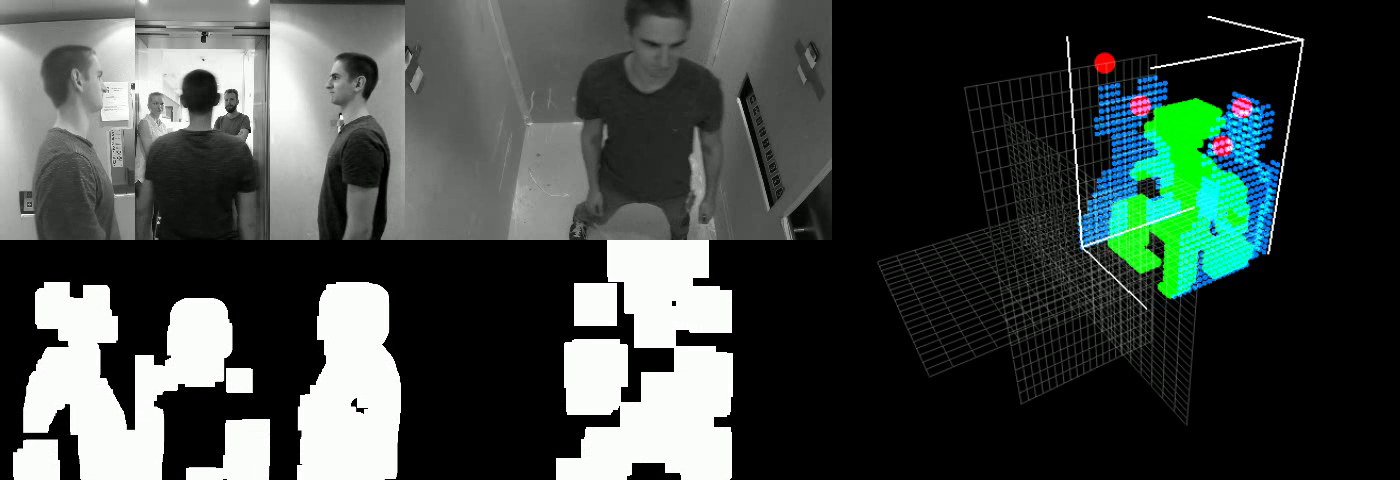
\includegraphics[width=1.0\textwidth, keepaspectratio]{volumeintersection_preview_04}
    
    \vspace{0.5em}
    
    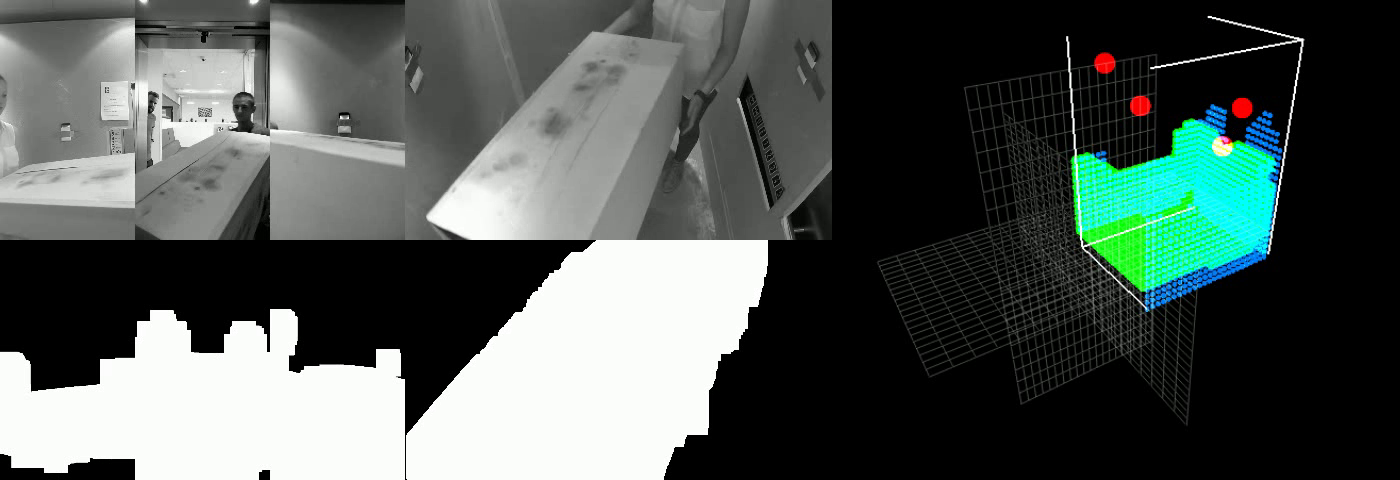
\includegraphics[width=1.0\textwidth, keepaspectratio]{volumeintersection_preview_03}
    
    \vspace{0.5em}
    
    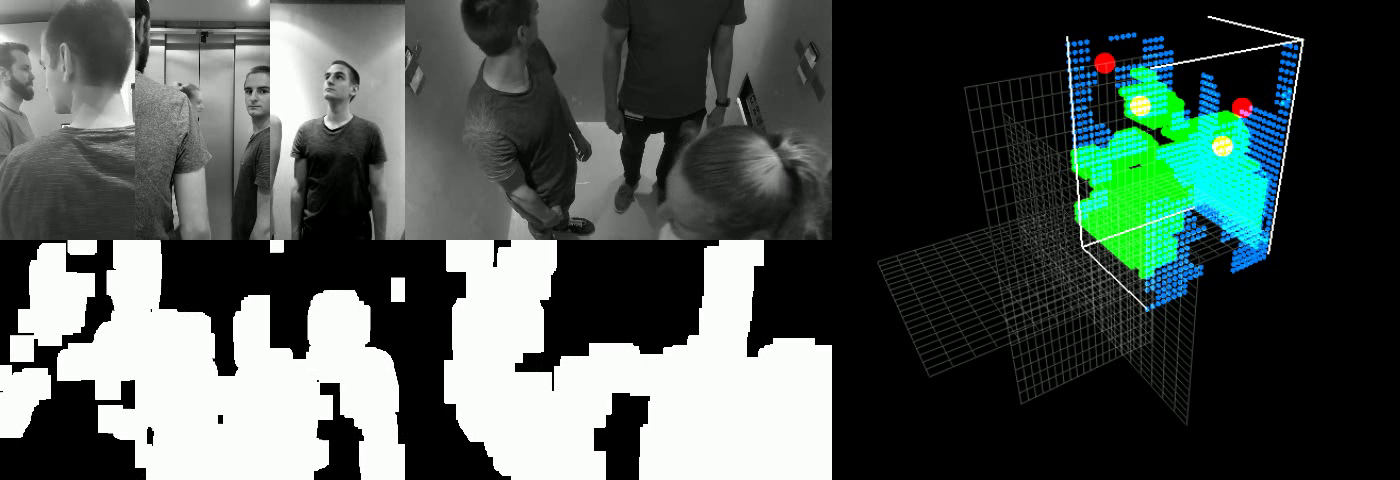
\includegraphics[width=1.0\textwidth, keepaspectratio]{volumeintersection_preview_05}
    
    \caption[Images of volume intersection test with orthogonal projection]{Images of volume intersection test with orthogonal projection. Each preview showing the camera images, foreground masks and the resulting volume intersection. (a) single passenger (b) cargo object (c) multiple passengers.}
    \label{fig:impl:videopreview}
\end{figure}

\subsection{Result Evaluation}
No ground truth for the volumetric data inside the cabin was recorded during the execution of the test.
This means the volume of the test subjects is unknown, as well as their position at every moment of time.
Therefore, here a qualitative evaluation is performed. 

The video capture works as intended.
However the choice of cameras resulted in a viewing angle, which did not cover the whole cabin.
This has the consequence that the corners of the cabin were not recorded an a passenger standing there was not registered by the system.
A wide angle camera on all sides might yield better results.

The foreground masking does not produce results of the desired quality.
It detects the passengers and cargo objects while they are moving.
However, often the center of the subject is not completely detected.
Only the outline and moving edged are recognized by the background subtractor.
This leads to \enquote{holes} in the reconstructed volume.
On the positive side of the adjustable parameters for the blur of the input image before the background subtraction and the adjustable amount of morphological opening and dilating of the foreground mask served good while experimenting with the footage.
In order to address the shortcomings of the foreground masking via background subtraction,
it could be possible to combine the technique with other image segmentation methods.

The volume reconstruction using a simple voxel-based method of volume intersection shows to be feasible in general for the purpose of life volume estimation, since no high accuracy is needed.
However the implemented orthogonal version is not completely correct, as a perspective projection would be needed.
Still it demonstrates general feasibility of this approach, 
as the orthogonal projection yields a volume description that is proportional but skewed.
Additionally, due to the holes in the foreground masks, these holes are also present in the volume image. 
This leads to inconsistencies.

The \ac{3D} blob detection and measurement has not been implemented as proposed.
This is a decision made in order to keep room for the 

- blob detection and measurement not implemented
- blob classification not feasable if blob quality is low because of viewving angle and holes
- conclusion: feasable, but needs a lot of work to be ready
- \ref{fig:impl:videopreview} shows the better parts, but most of the time there were holes
- video can also be found on CD / DVD

general concept feasible
small viewing angle: person out of frame
poor foreground separation by only applying background subtraction
non-correct orthogonal intersection implemented

TODO

\section{Scheduling Algorithm}
\subsection{Implementation of Simulation}
In section \ref{sec:design:schedulingalgorithm} the \emph{adaptive control strategy} has been introduced and an evaluation via a simulation has been planned.
This section describes the details of this implementation.

The simulation is implemented in the \emph{Rust} programming language.
Rust is a programming language initially developed by Mozilla.
According to its website it is a \enquote{systems programming language that runs blazingly fast, prevents segfaults, and guarantees thread safety} \autocite{rust2018rust}.
It features an expressive static type system and can be used to build applications that take advantage of modern hardware
\autocite[][]{matsakis2014rust}.
The rust compiler targets common platforms and operating and compiles source code to native machine code.
The language is chosen since the author is proficient in it.

The whole program spans over 880 lines of code.
It is not printed here but can be found on the attached CD or DVD.
Instead of printing it, its behavior and structure is explained in the following.

The \texttt{main} function is the entry point into the program.
In it, the general behavior of the simulation is defined.
It initializes the simulation parameters and traffic patterns and runs the actual simulation runs.
The actions it performs can be described as follows:
\begin{enumerate}
    \item Initialize the \texttt{BuildingParameters b}, \texttt{LiftParameters l} and\\ \texttt{SimulationParameters s}.
    \item Generate \texttt{s.simulations} many traffic \texttt{TrafficGenerator} instances, which each generates a traffic pattern. A traffic pattern describes the arrivals of traffic items for each tick of the simulation period. A Poisson distribution can be used to determine the number of traffic items that arrive within this tick \autocite{beers2015arrivals}.
    \item For each traffic patterns, run the simulation with the three different scheduling strategies. Each simulation is given the same parameters (\texttt{b, l, s}) and the same traffic pattern. The procedure to run a single simulation is described below.
    \item Collect the results of all simulations and filter out the results of any run, where any of the three strategies produced an invalid result.
    \item Calculate the specified metrics by aggregating all the results for each strategy.
\end{enumerate}
The implementation in Rust can be found in listing \ref{lst:app:simmain} in appendix \ref{app:sim}.

The actions taken in order to run a single simulation are then as follows:
\begin{enumerate}
    \item Create a new \texttt{ElevatorSystem e}, which holds the system state to be altered during the simulation.
    \item Create an empty \texttt{SimulationResults} metric container, which will aggregate the metrics for this run.
    \item While \texttt{e.ticks < s.total\_ticks()}, repeat the following simulation cycle:
    \begin{enumerate}
        \item Ask the control strategy for an action to be performed on the elevator system based on the current state of said system and the internal state of the control strategy.
        The action can be one of the actions listed as \texttt{ControlAction}.
        \item Perform the given action on the elevator system, thereby updating all fields effected by this action.
        \item Calculate the time it took to perform this action on the system and advance the ticks accordingly.
        \item Update the  metrics about waiting and ride time for each traffic item that is currently in the floor queues or in the elevator. Also update the metrics about the number of delivered traffic items and elevator stops.
        \item Copy the traffic item form the traffic pattern into the floor queues, which arrived in the time between the last tick and the updated tick.
    \end{enumerate}
    \item Correct the gathered metrics by removing the ride times of traffic items, who did not arrive at their destination yet and waiting times of traffic items, who did not yet enter the elevator.
\end{enumerate}
The implementation in Rust can be found in listing \ref{lst:app:simsinglerun} in appendix \ref{app:sim}.

The three control strategies are passed to the execution of a single simulation as generic parameters.
Therefore, they all implement an interface \texttt{ControlStrategy}.
A control strategy decides in each tick of the simulation, which action should be taken on the elevator system.
The behavior is the same as defined in section \ref{sec:design:schedulingalgorithms}, however, the actions such as \enquote{move elevator to floor X} are not performed in one action, but require instructions for the elevator system spanning over multiple ticks.
Hence, at each point in time and instruction from the \texttt{ControlAction} enumeration is given.

Figure \ref{fig:impl:simclass} shows a class diagram of the simulation program.
Rust is not a pure object-oriented language, but rather an imperative systems programming language, which solves generic programming via interfaces.
Therefore, the \ac{UML} class diagram is sub-optimal for the accurate representation of a Rust program.
It can still be used and gives a good overview of the types and instance variables present in the program.
Note that the \texttt{Main} class is not a class but a collection of functions.
It uses almost all of the types shown, even if no association is indicated in the diagram.

\begin{figure}[p]
    \centering
    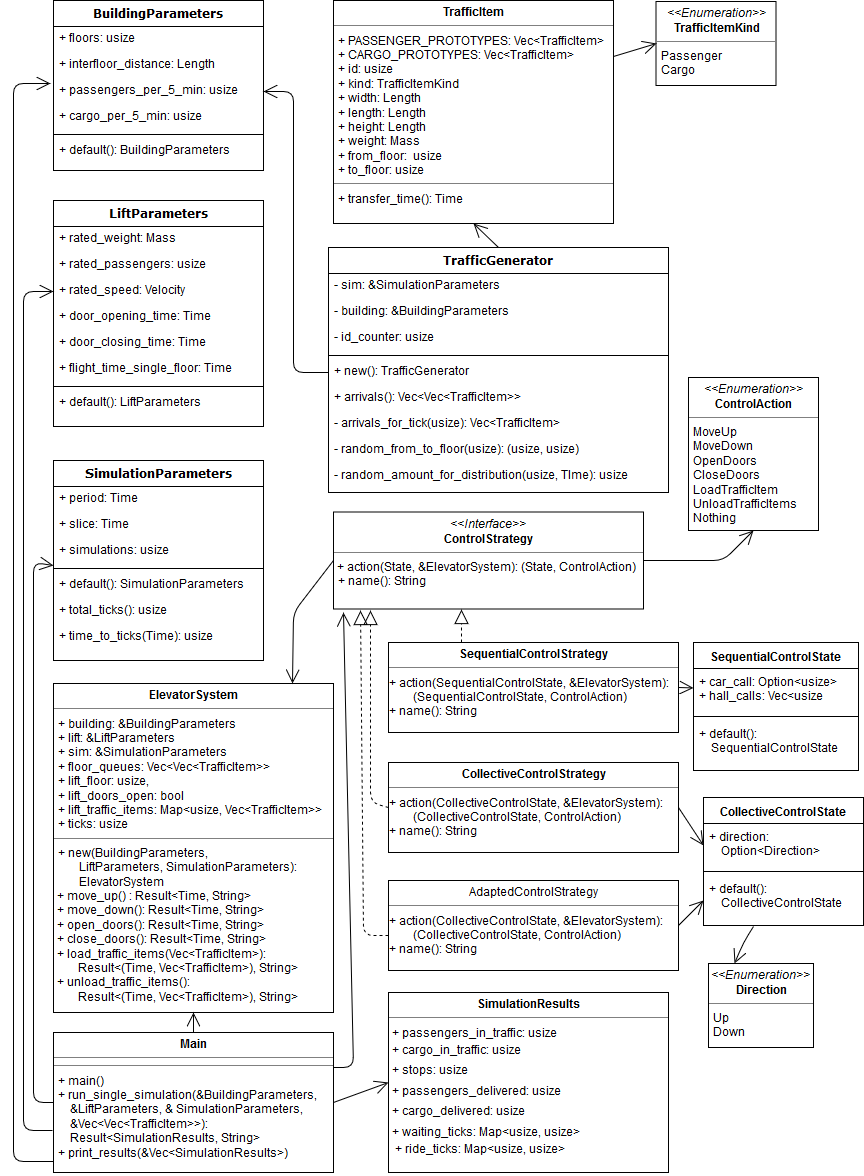
\includegraphics[width=1.0\textwidth, keepaspectratio]{sim_uml_class}
    \caption{Class diagram for the elevator simulation program}
    \label{fig:impl:simclass}
\end{figure}

The Rust implementation as a few dependencies, which are libraries used by the program.
All of them can be found in the rust package repository \autocite[][]{rust2018cratesio}.
This list describes their purpose in the program:
\begin{samepage}
\begin{itemize}[noitemsep]
    \item \texttt{lazy\_static}: Used for initialization of prototype list
    \item \texttt{rand}: Provides randomness functions and common likelihood functions including the Poisson distribution
    \item \texttt{rayon}: Provides data-driven multi-threading capabilities and is used to run the simulations in parallel
    \item \texttt{streaming-stats} (\texttt{stats}): Provides functions to create metrics with online algorithms such as average,  minimum, maximum and standard deviation
    \item \texttt{uom}: Provides types for units of measurements such as Mass and Time, as well as the respective \ac{SI} units such as kilograms and seconds
\end{itemize}
\end{samepage}

\subsection{Evaluation of Simulation Results}

\begingroup
\renewcommand*{\arraystretch}{1.0}
\begin{table}[]
\centering
\begin{tabular}{llrrr}
                                      &     & \begin{minipage}{2cm}\textbf{Sequential Control} \vspace{1em}\end{minipage} & \begin{minipage}{2cm}\textbf{Collective Control} \vspace{1em}\end{minipage} & \begin{minipage}{2cm}\textbf{Adaptive Control} \vspace{1em}\end{minipage}\\ \hline
\multirow{4}{*}{\textbf{Total passengers}}     & \textbf{min}        & 57.00                                                                                                                                             & 57.00                                                                                                                                             & 57.00                                                                                                                                           \\
                                               & \textbf{max}        & 113.00                                                                                                                                            & 113.00                                                                                                                                            & 113.00                                                                                                                                          \\
                                               & \textbf{avg}        & 84.09                                                                                                                                             & 84.09                                                                                                                                             & 84.09                                                                                                                                           \\
                                               & \textbf{$ \sigma $} & 8.97                                                                                                                                              & 8.97                                                                                                                                              & 8.97                                                                                                                                            \\ \hline
\multirow{4}{*}{\textbf{Total cargo}}          & \textbf{min}        & 9.00                                                                                                                                              & 9.00                                                                                                                                              & 9.00                                                                                                                                            \\
                                               & \textbf{max}        & 42.00                                                                                                                                             & 42.00                                                                                                                                             & 42.00                                                                                                                                           \\
                                               & \textbf{avg}        & 24.10                                                                                                                                             & 24.10                                                                                                                                             & 24.10                                                                                                                                           \\
                                               & \textbf{$ \sigma $} & 4.95                                                                                                                                              & 4.95                                                                                                                                              & 4.95                                                                                                                                            \\ \hline
\multirow{4}{*}{\textbf{Stops}}                & \textbf{min}        & 102.00                                                                                                                                            & 93.00                                                                                                                                             & 96.00                                                                                                                                           \\
                                               & \textbf{max}        & 135.00                                                                                                                                            & 158.00                                                                                                                                            & 157.00                                                                                                                                          \\
                                               & \textbf{avg}        & 118.47                                                                                                                                            & 125.75                                                                                                                                            & 129.60                                                                                                                                          \\
                                               & \textbf{$ \sigma $} & 5.22                                                                                                                                              & 10.41                                                                                                                                             & 9.30                                                                                                                                            \\ \hline
\multirow{4}{*}{\textbf{Passengers delivered}} & \textbf{min}        & 37.00                                                                                                                                             & 46.00                                                                                                                                             & 53.00                                                                                                                                           \\
                                               & \textbf{max}        & 65.00                                                                                                                                             & 107.00                                                                                                                                            & 108.00                                                                                                                                          \\
                                               & \textbf{avg}        & 49.32                                                                                                                                             & 78.06                                                                                                                                             & 79.67                                                                                                                                           \\
                                               & \textbf{$ \sigma $} & 4.24                                                                                                                                              & 9.45                                                                                                                                              & 8.75                                                                                                                                            \\ \hline
\multirow{4}{*}{\textbf{Cargo delivered}}      & \textbf{min}        & 3.00                                                                                                                                              & 3.00                                                                                                                                              & 4.00                                                                                                                                            \\
                                               & \textbf{max}        & 23.00                                                                                                                                             & 29.00                                                                                                                                             & 33.00                                                                                                                                           \\
                                               & \textbf{avg}        & 14.13                                                                                                                                             & 14.61                                                                                                                                             & 19.80                                                                                                                                           \\
                                               & \textbf{$ \sigma $} & 3.20                                                                                                                                              & 3.54                                                                                                                                              & 4.38                                                                                                                                            \\ \hline
\multirow{4}{*}{\textbf{Waiting time / s}}     & \textbf{min}        & 1.50                                                                                                                                              & 0.00                                                                                                                                              & 0.00                                                                                                                                            \\
                                               & \textbf{max}        & 2873.50                                                                                                                                           & 202.60                                                                                                                                            & 662.70                                                                                                                                          \\
                                               & \textbf{avg}        & 688.09                                                                                                                                            & 41.25                                                                                                                                             & 53.03                                                                                                                                           \\
                                               & \textbf{$ \sigma $} & 499.11                                                                                                                                            & 32.63                                                                                                                                             & 48.98                                                                                                                                           \\ \hline
\multirow{4}{*}{\textbf{Ride time / s}}        & \textbf{min}        & 13.00                                                                                                                                             & 13.00                                                                                                                                             & 13.00                                                                                                                                           \\
                                               & \textbf{max}        & 64.00                                                                                                                                             & 2180.20                                                                                                                                           & 1809.70                                                                                                                                         \\
                                               & \textbf{avg}        & 29.57                                                                                                                                             & 125.35                                                                                                                                            & 102.29                                                                                                                                          \\
                                               & \textbf{$ \sigma $} & 13.92                                                                                                                                             & 160.37                                                                                                                                            & 130.77                                                                                                                                         
\end{tabular}
\caption{\label{tab:impl:simulationresults} Simulation results for tested scheduling algorithms}
\end{table}
\endgroup

By running the implemented simulation, the results displayed in table \ref{tab:impl:simulationresults} are gathered.
It is visible that the three scheduling algorithms have distinct manifestations of the metrics that are recorded.
The sequential control sets focus on low ride time, the collective control sets focus on a balance between wait and ride time while maintaining a high delivery rate. 
The adaptive control strategy favors the delivery of cargo objects with lower ride times while trading for higher waiting times.
The key takeaways, expressed in relative numbers, here are:

\begin{itemize}
    \item Adaptive control delivers \textbf{more cargo items} on average than sequential control (\texttt{+}40.13~\%) and collective control (\texttt{+}35.52~\%).
    \item Collective control (\texttt{+}58.27~\%) and adaptive control (\texttt{+}61.53~\%) deliver \textbf{more passengers} on average compared to sequential control. 
    \item Sequential control shows a drastically higher mean waiting time then the other two (\texttt{+}1568.09~\%, \texttt{+}1297.55~\%). However, it features a lower average ride time (\texttt{-}76.41~\%, \texttt{-}71.09~\%), which is is only linear dependent on the travel distance.
    \item Adaptive control shows a slightly higher average waiting time (\texttt{+}30.56~\%) but has a lower (\texttt{-}18.40~\%) average ride time, which is less spread (\texttt{-}18.46~\%) compared to collective control.
\end{itemize}

In conclusion, these results for the adaptive control show, that giving cargo items priority and delivering them in a sequential style, while delivering passengers in a collective style, 
can increase the amount of cargo that gets delivered. 
This reduces the average ride time. 
However, it comes with a trade-off in waiting time.
The increased performance can be explained by the reduced time, 
the cargo items block the space and weight restrictions present in the elevator cabin and prevent other passengers from entering.
Therefore delivering them faster causes a shorter blocking of these resources, resulting in better overall utilization.

The precondition of applying the adaptive control strategy is the knowledge, 
whether a cargo object is currently inside the elevator cabin and is blocking it for other passengers 
and the information about the destination of this object.
This information can be obtained by combining the visual system presented before, which is capable of detecting cargo objects by their volume, with the information about car calls made for this object. To create the association of an object present in the lift and its destination, 
the time of entering the cabin and performing the car call can be correlated.
Otherwise, in an environment that features hall calls with information about the destination, this association can be used.
An alternative would be an \emph{override} button in the cabin, 
to give priority to the current car call, regardless of the presence of a cargo object in the cabin.

However, the scenario chosen for the simulation is very specific and can benefit from the kinds of optimizations the adaptive control yields. 
The given traffic conditions in a multi-storey building with a single elevator, 
which is used by passengers and cargo alike, 
do favor the prioritization of cargo items by sequentially delivering them.
The results for other traffic patterns, e.g. for elevators that only convey passengers,
might differ and might not benefit from adapted scheduling.

\section{Economic Considerations}
As stated above, the presented scheduling algorithm can use the visual system to determine the presence of a cargo object, which can benefit the handling capacity of elevators which are regularly used by passengers and cargo items.
There are several possible real-life scenarios with these properties:
\begin{itemize}
    \item \textbf{Hospitals} with elevators where patient beds are moved. The medical beds are usually as large as the elevator allows and therefore block the elevator from being used by groups of additional passengers. Additionally, patients with medical conditions who occupy the bed often should have a prioritized transport, as their health might depend on every second spent in the elevator. 
    \item Large office buildings with \textbf{auxiliary lifts} that are used by janitors and craftsman, who carry carts, tool cabinets or hardware material. These lifts could also be used by regular passengers and might even be integrated into an elevator group. However, the cart could block the elevator.
    \item Multi-storey \textbf{Warehouses} or \textbf{fabrication plants} with heavy duty cargo lifts used 
    by factory employees and forklifts or other transportation devices for heavy goods. The lifts block each other from entering the lift and therefore need to be handled sequentially. 
\end{itemize}

Possible customers for DXC Technology and the Digital Service Innovation team are Otis, Kone, Schindler and Thyssen, which \textcite[][p.~4]{unger2015aufzuege} identifies as the biggest elevator companies. Some of those companies already have business relations with DXC Technology and therefore might be interested in setting up an innovative project to explore the ideas presented in this paper.
They could consider offering an elevator system with an integrated visual system to customers with the needs described above, who construct a new building or want to upgrade an existing lift, as an optional feature at an additional charge.

The cost structure for the visual solution is threefold. 
A project implementing this or a similar solution generates cost during development, installation of the individual solution and later operation.
Since elevator technology experts and computer vision experts need to work together for the development of an advanced visual solution in elevators, 
the costs in this phase are characterized by expenses for said experts, as well as laboratory equipment.
Developing resilient and high-quality software requires careful planning and implementation and is therefore crucial for the costs at this stage.
When installing the  solution into an elevator cabin and integrating it into the control circuit, the costs are governed by the hardware installed and the labor of the technician installing it. 
The costs for the hardware includes multiple cameras, do neither need an extraordinary high resolution nor frame rate, and a general purpose computer to process the images, which needs to have enough computing power to process the images in near real-time. 
Furthermore, a connection to the elevator controller is necessary which might require some kind of adapter.
During operation, the costs are reduced down to the electricity consumed by the additional components and  the costs for maintaining the system.

Possible savings from implementing the proposed visual system and the scheduling algorithm manifest in the faster delivery of cargo items and therefore the reduction of the time they block the cabin for other passengers. 
This can result in a higher overall passenger throughput and therefore reduce the energy needs per passenger.
Furthermore, the faster delivery of cargo objects can have impacts on the costs associated with their travel time, which highly depend on the type of good that is transported and the environment it is situated in. 
For example in a production plant, reduced transport times for the produced goods could lead to reduced production costs in general.


\section{Privacy Considerations}
Installing a camera system unavoidably raises privacy and security concerns 
for the filmed individuals.
Especially in elevators, which are publicly accessible, there are legal requirements to fulfill.
In Germany the Federal Data Protection Act, \\
\ac{BDSG} \autocite[][]{bmjv2009bdsg}, 
regulates the usage of video surveillance systems.
Public areas may only be observed for specified purposes.
The presence of a surveillance system must be indicated,
as well as the name and contact of its controller. 
When the data gathered by the system is no longer needed for the specified purpose, it must be deleted 
\autocite[][§~4]{bmjv2009bdsg}.
The European \ac{GDPR} \autocite{eu2016gdpr} describes similar, more broad principles:  
\emph{data transparency, purpose limitation, data minimization, storage limitation and confidentiality}
\autocite{ico2018gdpr}.
Oriented at this principle the following paragraphs provide privacy consideration about the visual system.

The presented visual system has a \emph{limited purpose}, in that it is only used 
to determine whether passengers or cargo items are present in the elevator cabin 
and what volume they take up. 
This information is used to improve the scheduling of the elevator.

In order to keep the usage of video data \emph{transparent},
passengers should be informed about the video system before they enter the cabin.
This could be done by installing a sign, which indicates the presence of the video system, 
clearly states, for what purpose the video data is used for, 
and who is operating the system and can be contacted in case of issues.
The sign should be in front and inside of the elevator, 
so that potential passengers can decide,
if they want to use the lift and be filmed.

Since the system has a limited purpose, 
only data specific to that purpose should be gathered and processed.
The data usage should be \emph{minimized}.
Only as few cameras as possible, but as many as necessary should be installed in the lift.
Areas that are not of interest for the lift system should not be filmed.
Furthermore, the resolution of the cameras should be only as high as necessary.
For purpose of detecting the presence, position, and outline of a passenger or cargo object 
in the cabin, it is not required to capture fine details.
The DIN EN 62676-4 norm \autocite[][]{din2016surveillance} recommends 
to use a camera resolution, which captures 25 to 62.5 pixel per meter,
for the purpose of detecting or monitoring people.
In addition, the kind of processing of the video data should be limited to the extent necessary for the purpose of the video system. 
For example, it is not necessary to perform face detection  or to identify individuals.
However, tracking the path of an individual over the course of their journey might be beneficial for the application.

The presented system can operate in real time.
Only the current video frame is needed to determine the presence and volume of passengers and objects.
Therefore, the \emph{storage} of the video data can be \emph{limited}.
There is no need to store the video data at all.

In order to keep the video data \emph{confidential}, 
measures must be taken to prevent access by unauthorized parties.
For the purpose of the system, all data processing can be done locally within the elevator system.
The visual system only needs to interact with the elevator controller.
Therefore there is no need to make the data available to the outside, e.g. the internet.
Doing so would open up unnecessary possibilities for misuse of the video system.
